
\begin{figure}[t]
    % \vspace{-2em}
    \centering
    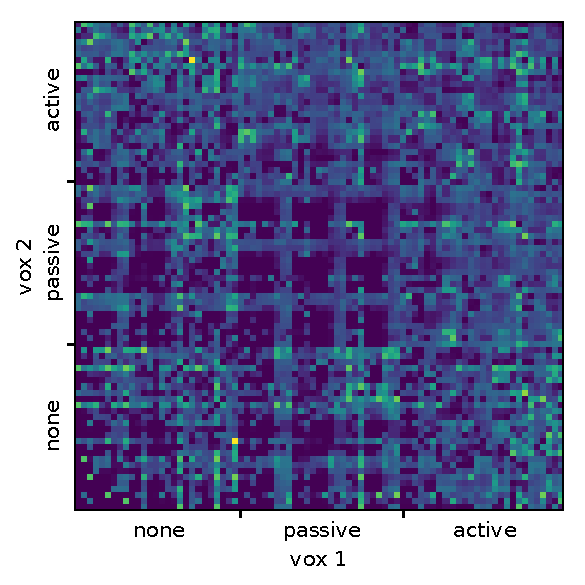
\includegraphics[width=0.7\linewidth]{Chapter02/fig/design_space.pdf}
    % \vspace{-2em}
    \caption{\textbf{Simulating modular soft robots.}
    The design space is plotted as a heatmap, containing one cell for each of the 6561 possible configurations.
    Lighter colored cells are fitter designs (Eq.~\ref{eq:fitness}).
    Each design is defined by a vector of eight ternary values, indicating what kind of voxel (none, passive, or active) the design contains at the eight lattice points in the $2\times2\times2$ workspace.
    The 8D ternary vector is reduced to a 2D heatmap by nesting pairs of dimensions within each other: four, nested $3\times3$ grids result in a $3^4\times3^4=81\times81$ overall heatmap.
    }
    \label{fig:sim}
    % \vspace{-1em}
\end{figure}
